%\VignetteEngine{knitr::knitr}
%\VignetteIndexEntry{Grade of Membership Clustering and Visualization using CountClust}
%\VignettePackage{CountClust}

% To compile this document
% library('knitr'); rm(list=ls()); knit('CountClust/vignettes/count-clust.Rnw')
% library('knitr'); rm(list=ls()); knit2pdf('CountClust/vignettes/count-clust.Rnw'); openPDF('count-clust.pdf')
% !Rnw weave = knitr

\documentclass[12pt]{article}\usepackage[]{graphicx}\usepackage[usenames,dvipsnames]{color}
%% maxwidth is the original width if it is less than linewidth
%% otherwise use linewidth (to make sure the graphics do not exceed the margin)
\makeatletter
\def\maxwidth{ %
  \ifdim\Gin@nat@width>\linewidth
    \linewidth
  \else
    \Gin@nat@width
  \fi
}
\makeatother

\definecolor{fgcolor}{rgb}{0.345, 0.345, 0.345}
\newcommand{\hlnum}[1]{\textcolor[rgb]{0.686,0.059,0.569}{#1}}%
\newcommand{\hlstr}[1]{\textcolor[rgb]{0.192,0.494,0.8}{#1}}%
\newcommand{\hlcom}[1]{\textcolor[rgb]{0.678,0.584,0.686}{\textit{#1}}}%
\newcommand{\hlopt}[1]{\textcolor[rgb]{0,0,0}{#1}}%
\newcommand{\hlstd}[1]{\textcolor[rgb]{0.345,0.345,0.345}{#1}}%
\newcommand{\hlkwa}[1]{\textcolor[rgb]{0.161,0.373,0.58}{\textbf{#1}}}%
\newcommand{\hlkwb}[1]{\textcolor[rgb]{0.69,0.353,0.396}{#1}}%
\newcommand{\hlkwc}[1]{\textcolor[rgb]{0.333,0.667,0.333}{#1}}%
\newcommand{\hlkwd}[1]{\textcolor[rgb]{0.737,0.353,0.396}{\textbf{#1}}}%
\let\hlipl\hlkwb

\usepackage{framed}
\makeatletter
\newenvironment{kframe}{%
 \def\at@end@of@kframe{}%
 \ifinner\ifhmode%
  \def\at@end@of@kframe{\end{minipage}}%
  \begin{minipage}{\columnwidth}%
 \fi\fi%
 \def\FrameCommand##1{\hskip\@totalleftmargin \hskip-\fboxsep
 \colorbox{shadecolor}{##1}\hskip-\fboxsep
     % There is no \\@totalrightmargin, so:
     \hskip-\linewidth \hskip-\@totalleftmargin \hskip\columnwidth}%
 \MakeFramed {\advance\hsize-\width
   \@totalleftmargin\z@ \linewidth\hsize
   \@setminipage}}%
 {\par\unskip\endMakeFramed%
 \at@end@of@kframe}
\makeatother

\definecolor{shadecolor}{rgb}{.97, .97, .97}
\definecolor{messagecolor}{rgb}{0, 0, 0}
\definecolor{warningcolor}{rgb}{1, 0, 1}
\definecolor{errorcolor}{rgb}{1, 0, 0}
\newenvironment{knitrout}{}{} % an empty environment to be redefined in TeX

\usepackage{alltt}

\newcommand{\CountClust}{\textit{CountClust}}
\usepackage{dsfont}
\usepackage{cite}




\RequirePackage{/Library/Frameworks/R.framework/Versions/3.3/Resources/library/BiocStyle/resources/tex/Bioconductor}

\AtBeginDocument{\bibliographystyle{/Library/Frameworks/R.framework/Versions/3.3/Resources/library/BiocStyle/resources/tex/unsrturl}}


\author{Kushal K Dey, Chiaowen Joyce Hsiao \& Matthew Stephens \\[1em] \small{\textit{Stephens Lab}, The University of Chicago} \mbox{ }\\ \small{\texttt{$^*$Correspondending Email: mstephens@uchicago.edu}}}

\bioctitle[Grade of Membership Clustering and Visualization using \CountClust{}]{Grade of Membership Model and Visualization for RNA-seq data using \CountClust{}}
\IfFileExists{upquote.sty}{\usepackage{upquote}}{}
\begin{document}

\maketitle

\begin{abstract}
  \vspace{1em}
 Grade of membership or GoM models (also known as admixture models or Latent Dirichlet Allocation") are a generalization of cluster models that allow each sample to have membership in multiple clusters. It is widely used to model ancestry of individuals in population genetics based on SNP/ microsatellite data and also in natural language processing for modeling documents \cite{Pritchard2000, Blei2003}.

This \R{} package implements tools to visualize the clusters obtained from fitting topic models using a Structure plot \cite{Rosenberg2002} and extract the top features/genes that distinguish the clusters. In presence of known technical or batch effects, the package also allows for correction of these confounding effects.

\vspace{1em}
\textbf{\CountClust{} version:} 0.1.2 \footnote{This document used the vignette from \Bioconductor{} package \Biocpkg{DESeq2, cellTree} as \CRANpkg{knitr} template}
\end{abstract}




\newpage

\tableofcontents

\section{Introduction}

In the context of RNA-seq expression (bulk or singlecell seq) data, the grade of membership model allows each sample (usually a tissue sample or a single cell) to have some proportion of its RNA-seq reads coming from each cluster. For typical bulk RNA-seq experiments this assumption
can be argued as follows: each tissue sample is a mixture of different cell types, and so clusters could represent cell types (which are determined by the expression patterns of the genes), and the membership of a sample in each cluster could represent the proportions of each cell type present in that sample.

Many software packages available for document clustering are applicable to modeling RNA-seq data. Here, we use the R package {\tt maptpx} \cite{Taddy2012} to fit these models, and add functionality for visualizing the results and annotating clusters by their most distinctive genes to help biological interpretation. We also provide additional functionality to correct for batch effects and also compare the outputs from two different grade of membership model fits to the same set of samples but different in terms of feature description or model assumptions.

\section{\CountClust{} Installation}

\CountClust{} requires the following CRAN-R packages: \CRANpkg{maptpx}, \CRANpkg{ggplot2}, \CRANpkg{cowplot}, \CRANpkg{parallel}, \CRANpkg{reshape2}, \CRANpkg{RColorBrewer}, \CRANpkg{flexmix}, \CRANpkg{gtools}, \CRANpkg{devtools} along with the \Bioconductor{} package: \Biocpkg{limma}.

\begin{knitrout}
\definecolor{shadecolor}{rgb}{0.969, 0.969, 0.969}\color{fgcolor}\begin{kframe}
\begin{alltt}
\hlkwd{source}\hlstd{(}\hlstr{"http://bioconductor.org/biocLite.R"}\hlstd{)}
\hlkwd{biocLite}\hlstd{(}\hlstr{"CountClust"}\hlstd{)}
\end{alltt}
\end{kframe}
\end{knitrout}

For the latest updated version of the package \begin{verb} maptpx \end{verb} package (with some bug fixes from the CRAN version), we recommend the user to install the Github version.

\begin{knitrout}
\definecolor{shadecolor}{rgb}{0.969, 0.969, 0.969}\color{fgcolor}\begin{kframe}
\begin{alltt}
\hlkwd{library}\hlstd{(devtools)}
\hlkwd{install_github}\hlstd{(}\hlstr{"kkdey/maptpx"}\hlstd{)}
\end{alltt}
\end{kframe}
\end{knitrout}

The working version of the \CountClust{} package is available on Github, along with the data packages used as examples in this vignette.

\begin{knitrout}
\definecolor{shadecolor}{rgb}{0.969, 0.969, 0.969}\color{fgcolor}\begin{kframe}
\begin{alltt}
\hlkwd{install_github}\hlstd{(}\hlstr{'kkdey/CountClust'}\hlstd{)}
\end{alltt}
\end{kframe}
\end{knitrout}

Then load the package with:

\begin{knitrout}
\definecolor{shadecolor}{rgb}{0.969, 0.969, 0.969}\color{fgcolor}\begin{kframe}
\begin{alltt}
\hlkwd{library}\hlstd{(CountClust)}
\end{alltt}
\end{kframe}
\end{knitrout}

\section{Data Preparation}

We install data packages as \begin{verb} expressionSet \end{verb} objects for bulk RNA-seq reads data from Brain tissue samples of human donors under GTEx (Genotype Tissue Expression) V6 Project  \cite{GTEX2013} and a singlecell RNA-seq reads data across developmental stages in mouse embryo due to Deng \textit{et al} 2014 \cite{Deng2014}.

%The data package due to Deng \textit{et al} is a processed version of the data publicly available at Gene Expression Omnibus (GEO:GSE45719: see \url{http://www.ncbi.nlm.nih.gov/geo/query/acc.cgi?acc=GSE45719}).

\begin{verb} singleCellRNASeqMouseDeng2014 \end{verb} data package due to Deng \textit{et al} is a processed version of the data publicly available at Gene Expression Omnibus (GEO:GSE45719: see \url{http://www.ncbi.nlm.nih.gov/geo/query/acc.cgi?acc=GSE45719}).

%The data package for GTEx V6 Brain sample data is again a processed version of the data publicly available at the GTEx Portal (\url{http://www.gtexportal.org/home/}, dbGaP accession phs000424.v6.p1, release date: Oct 19, 2015).

\begin{knitrout}
\definecolor{shadecolor}{rgb}{0.969, 0.969, 0.969}\color{fgcolor}\begin{kframe}
\begin{alltt}
\hlkwd{library}\hlstd{(devtools)}

\hlstd{read.data1} \hlkwb{=} \hlkwa{function}\hlstd{() \{}
  \hlstd{x} \hlkwb{=} \hlkwd{tempfile}\hlstd{()}
  \hlkwd{download.file}\hlstd{(}\hlstr{'https://cdn.rawgit.com/kkdey/singleCellRNASeqMouseDeng2014/master/data/Deng2014MouseEsc.rda'}\hlstd{,} \hlkwc{destfile}\hlstd{=x,} \hlkwc{quiet}\hlstd{=}\hlnum{TRUE}\hlstd{)}
  \hlstd{z} \hlkwb{=} \hlkwd{get}\hlstd{(}\hlkwd{load}\hlstd{((x)))}
  \hlkwd{return}\hlstd{(z)}
\hlstd{\}}

\hlstd{Deng2014MouseESC} \hlkwb{<-} \hlkwd{read.data1}\hlstd{()}

\hlcom{## Alternatively}
\hlcom{# install_github('kkdey/singleCellRNASeqMouseDeng2014')}
\end{alltt}
\end{kframe}
\end{knitrout}

\begin{verb} GTExV6Brain \end{verb} The data package for GTEx V6 Brain sample data is again a processed version of the data publicly available at the GTEx Portal (\url{http://www.gtexportal.org/home/}, dbGaP accession phs000424.v6.p1, release date: Oct 19, 2015).

\begin{knitrout}
\definecolor{shadecolor}{rgb}{0.969, 0.969, 0.969}\color{fgcolor}\begin{kframe}
\begin{alltt}
\hlstd{read.data2} \hlkwb{=} \hlkwa{function}\hlstd{() \{}
  \hlstd{x} \hlkwb{=} \hlkwd{tempfile}\hlstd{()}
  \hlkwd{download.file}\hlstd{(}\hlstr{'https://cdn.rawgit.com/kkdey/GTExV6Brain/master/data/GTExV6Brain.rda'}\hlstd{,} \hlkwc{destfile} \hlstd{= x,} \hlkwc{quiet}\hlstd{=}\hlnum{TRUE}\hlstd{)}
  \hlstd{z} \hlkwb{=} \hlkwd{get}\hlstd{(}\hlkwd{load}\hlstd{((x)))}
  \hlkwd{return}\hlstd{(z)}
\hlstd{\}}

\hlstd{GTExV6Brain} \hlkwb{<-} \hlkwd{read.data2}\hlstd{()}

\hlcom{## Alternatively}
\hlcom{# install_github('kkdey/GTExV6Brain')}
\end{alltt}
\end{kframe}
\end{knitrout}

\subsubsection{Deng et al 2014}

Load the scRNA-seq data due to Deng \textit{et al} 2014.

\begin{knitrout}
\definecolor{shadecolor}{rgb}{0.969, 0.969, 0.969}\color{fgcolor}\begin{kframe}
\begin{alltt}
\hlstd{deng.counts} \hlkwb{<-} \hlstd{Biobase}\hlopt{::}\hlkwd{exprs}\hlstd{(Deng2014MouseESC)}
\hlstd{deng.meta_data} \hlkwb{<-} \hlstd{Biobase}\hlopt{::}\hlkwd{pData}\hlstd{(Deng2014MouseESC)}
\hlstd{deng.gene_names} \hlkwb{<-} \hlkwd{rownames}\hlstd{(deng.counts)}
\end{alltt}
\end{kframe}
\end{knitrout}

\subsubsection{GTEx V6 Brain}

Load the bulk-RNA seq data from GTEx V6 brain data.

\begin{knitrout}
\definecolor{shadecolor}{rgb}{0.969, 0.969, 0.969}\color{fgcolor}\begin{kframe}
\begin{alltt}
\hlstd{gtex.counts} \hlkwb{<-} \hlstd{Biobase}\hlopt{::}\hlkwd{exprs}\hlstd{(GTExV6Brain)}
\hlstd{gtex.meta_data} \hlkwb{<-} \hlstd{Biobase}\hlopt{::}\hlkwd{pData}\hlstd{(GTExV6Brain)}
\hlstd{gtex.gene_names} \hlkwb{<-} \hlkwd{rownames}\hlstd{(gtex.counts)}
\end{alltt}
\end{kframe}
\end{knitrout}


\section{Fitting the GoM Model}

We use a wrapper function of the \textit{topics()} function in the \CRANpkg{maptpx} due to Matt Taddy \cite{Taddy2012}.

As an example, we fit the topic model for \Robject{k}=4 on the GTEx V6 Brain data and save the GoM model output file to user-defined directory.

\begin{knitrout}
\definecolor{shadecolor}{rgb}{0.969, 0.969, 0.969}\color{fgcolor}\begin{kframe}
\begin{alltt}
\hlkwd{FitGoM}\hlstd{(}\hlkwd{t}\hlstd{(gtex.counts),}
            \hlkwc{K}\hlstd{=}\hlnum{4}\hlstd{,} \hlkwc{tol}\hlstd{=}\hlnum{0.1}\hlstd{,}
            \hlkwc{path_rda}\hlstd{=}\hlstr{"../data/GTExV6Brain.FitGoM.rda"}\hlstd{)}
\end{alltt}
\end{kframe}
\end{knitrout}

One can also input a vector of clusters under \begin{verb} nclus_vec \end{verb} as we do for a list of cluster numbers from $2$ to $7$ for Deng \textit{et al} 2014 data.

\begin{knitrout}
\definecolor{shadecolor}{rgb}{0.969, 0.969, 0.969}\color{fgcolor}\begin{kframe}
\begin{alltt}
\hlkwd{FitGoM}\hlstd{(}\hlkwd{t}\hlstd{(deng.counts),}
            \hlkwc{K}\hlstd{=}\hlnum{2}\hlopt{:}\hlnum{7}\hlstd{,} \hlkwc{tol}\hlstd{=}\hlnum{0.1}\hlstd{,}
            \hlkwc{path_rda}\hlstd{=}\hlstr{"../data/MouseDeng2014.FitGoM.rda"}\hlstd{)}
\end{alltt}
\end{kframe}
\end{knitrout}



\section{Structure plot visualization}

Now we perform the visualization for \Robject{k}=$6$ for the Deng \textit{et al} 2014 data.

We load the GoM fit for \Robject{k}=6.

\begin{knitrout}
\definecolor{shadecolor}{rgb}{0.969, 0.969, 0.969}\color{fgcolor}\begin{kframe}
\begin{alltt}
\hlkwd{data}\hlstd{(}\hlstr{"MouseDeng2014.FitGoM"}\hlstd{)}
\hlkwd{names}\hlstd{(MouseDeng2014.FitGoM}\hlopt{$}\hlstd{clust_6)}
\end{alltt}
\begin{verbatim}
## [1] "K"     "theta" "omega" "BF"    "D"     "X"
\end{verbatim}
\begin{alltt}
\hlstd{omega} \hlkwb{<-} \hlstd{MouseDeng2014.FitGoM}\hlopt{$}\hlstd{clust_6}\hlopt{$}\hlstd{omega}
\end{alltt}
\end{kframe}
\end{knitrout}

We prepare the annotations for the visualization.

\begin{knitrout}
\definecolor{shadecolor}{rgb}{0.969, 0.969, 0.969}\color{fgcolor}\begin{kframe}
\begin{alltt}
\hlstd{annotation} \hlkwb{<-} \hlkwd{data.frame}\hlstd{(}
  \hlkwc{sample_id} \hlstd{=} \hlkwd{paste0}\hlstd{(}\hlstr{"X"}\hlstd{,} \hlkwd{c}\hlstd{(}\hlnum{1}\hlopt{:}\hlkwd{NROW}\hlstd{(omega))),}
  \hlkwc{tissue_label} \hlstd{=} \hlkwd{factor}\hlstd{(}\hlkwd{rownames}\hlstd{(omega),}
                        \hlkwc{levels} \hlstd{=} \hlkwd{rev}\hlstd{(} \hlkwd{c}\hlstd{(}\hlstr{"zy"}\hlstd{,} \hlstr{"early2cell"}\hlstd{,}
                                        \hlstr{"mid2cell"}\hlstd{,} \hlstr{"late2cell"}\hlstd{,}
                                        \hlstr{"4cell"}\hlstd{,} \hlstr{"8cell"}\hlstd{,} \hlstr{"16cell"}\hlstd{,}
                                        \hlstr{"earlyblast"}\hlstd{,}\hlstr{"midblast"}\hlstd{,}
                                         \hlstr{"lateblast"}\hlstd{) ) ) )}

\hlkwd{rownames}\hlstd{(omega)} \hlkwb{<-} \hlstd{annotation}\hlopt{$}\hlstd{sample_id;}
\end{alltt}
\end{kframe}
\end{knitrout}

Now we perform the visualization.

\begin{figure}[htp]
\begin{center}
\begin{knitrout}
\definecolor{shadecolor}{rgb}{0.969, 0.969, 0.969}\color{fgcolor}\begin{kframe}
\begin{alltt}
\hlkwd{StructureGGplot}\hlstd{(}\hlkwc{omega} \hlstd{= omega,}
                \hlkwc{annotation} \hlstd{= annotation,}
                \hlkwc{palette} \hlstd{= RColorBrewer}\hlopt{::}\hlkwd{brewer.pal}\hlstd{(}\hlnum{8}\hlstd{,} \hlstr{"Accent"}\hlstd{),}
                \hlkwc{yaxis_label} \hlstd{=} \hlstr{"Development Phase"}\hlstd{,}
                \hlkwc{order_sample} \hlstd{=} \hlnum{TRUE}\hlstd{,}
                \hlkwc{axis_tick} \hlstd{=} \hlkwd{list}\hlstd{(}\hlkwc{axis_ticks_length} \hlstd{=} \hlnum{.1}\hlstd{,}
                                 \hlkwc{axis_ticks_lwd_y} \hlstd{=} \hlnum{.1}\hlstd{,}
                                 \hlkwc{axis_ticks_lwd_x} \hlstd{=} \hlnum{.1}\hlstd{,}
                                 \hlkwc{axis_label_size} \hlstd{=} \hlnum{7}\hlstd{,}
                                 \hlkwc{axis_label_face} \hlstd{=} \hlstr{"bold"}\hlstd{))}
\end{alltt}
\end{kframe}
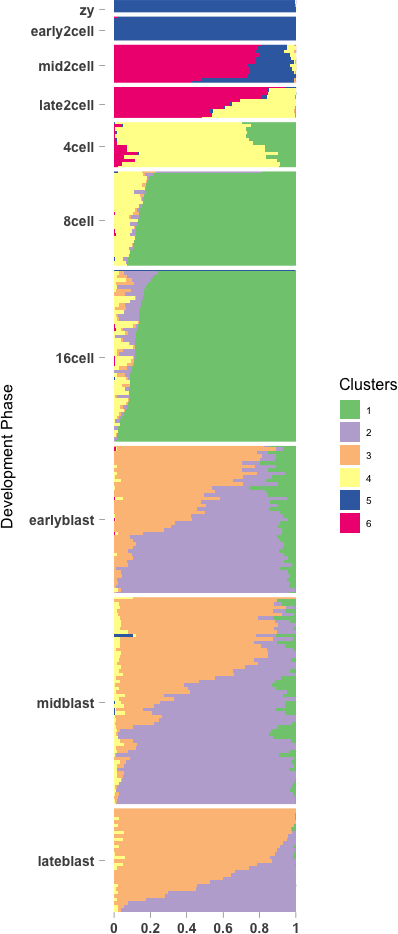
\includegraphics[width=3in,height=7in]{figure/plot_topic_deng-1} 

\end{knitrout}
\end{center}
\end{figure}

%\begin{figure}[htp]
%\begin{center}
%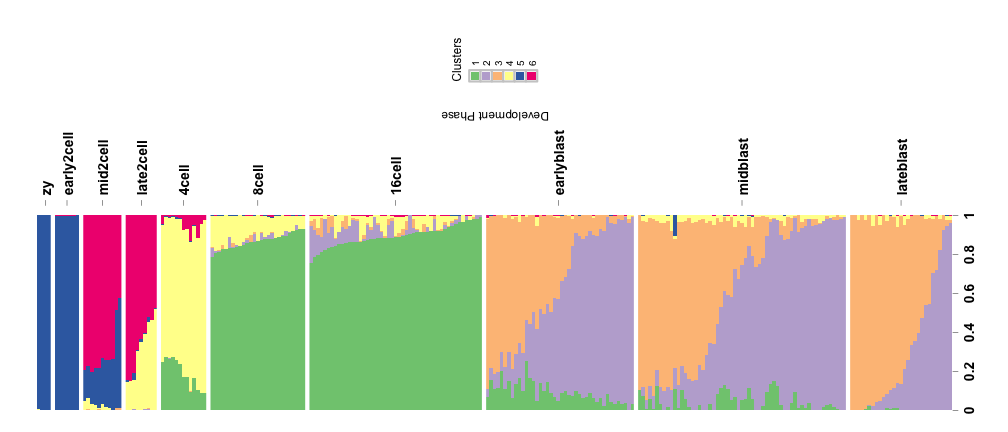
\includegraphics[width=3in,height=7in]{figures/plot_topic_deng-1}
%\end{center}
%\end{figure}

In the above plot, the samples in each batch have been sorted by the proportional memebership of the most representative cluster in that batch. One can also use \begin{verb} order_sample=FALSE \end{verb} for the un-ordered version, which retains the order as in the data (see Supplementary analysis for example).

Now we perform the Structure plot visualization for \Robject{k}=$4$ for GTEx V6 data for Brain samples .

We load the GoM fit for \Robject{k}=4.

\begin{knitrout}
\definecolor{shadecolor}{rgb}{0.969, 0.969, 0.969}\color{fgcolor}\begin{kframe}
\begin{alltt}
\hlkwd{data}\hlstd{(}\hlstr{"GTExV6Brain.FitGoM"}\hlstd{)}
\hlstd{omega} \hlkwb{<-} \hlstd{GTExV6Brain.FitGoM}\hlopt{$}\hlstd{omega;}
\hlkwd{dim}\hlstd{(omega)}
\end{alltt}
\begin{verbatim}
## [1] 1259    4
\end{verbatim}
\begin{alltt}
\hlkwd{colnames}\hlstd{(omega)} \hlkwb{<-} \hlkwd{c}\hlstd{(}\hlnum{1}\hlopt{:}\hlkwd{NCOL}\hlstd{(omega))}
\end{alltt}
\end{kframe}
\end{knitrout}

We now prepare the annotations for the visualization.

\begin{knitrout}
\definecolor{shadecolor}{rgb}{0.969, 0.969, 0.969}\color{fgcolor}\begin{kframe}
\begin{alltt}
\hlstd{tissue_labels} \hlkwb{<-} \hlstd{gtex.meta_data[,}\hlnum{3}\hlstd{];}


\hlstd{annotation} \hlkwb{<-} \hlkwd{data.frame}\hlstd{(}
    \hlkwc{sample_id} \hlstd{=} \hlkwd{paste0}\hlstd{(}\hlstr{"X"}\hlstd{,} \hlnum{1}\hlopt{:}\hlkwd{length}\hlstd{(tissue_labels)),}
    \hlkwc{tissue_label} \hlstd{=} \hlkwd{factor}\hlstd{(tissue_labels,}
                          \hlkwc{levels} \hlstd{=} \hlkwd{rev}\hlstd{(}\hlkwd{unique}\hlstd{(tissue_labels) ) ) );}

\hlstd{cols} \hlkwb{<-} \hlkwd{c}\hlstd{(}\hlstr{"blue"}\hlstd{,} \hlstr{"darkgoldenrod1"}\hlstd{,} \hlstr{"cyan"}\hlstd{,} \hlstr{"red"}\hlstd{)}
\end{alltt}
\end{kframe}
\end{knitrout}

Now we perform the visualization.

\begin{knitrout}
\definecolor{shadecolor}{rgb}{0.969, 0.969, 0.969}\color{fgcolor}\begin{kframe}
\begin{alltt}
\hlkwd{StructureGGplot}\hlstd{(}\hlkwc{omega} \hlstd{= omega,}
                \hlkwc{annotation}\hlstd{= annotation,}
                \hlkwc{palette} \hlstd{= cols,}
                \hlkwc{yaxis_label} \hlstd{=} \hlstr{""}\hlstd{,}
                \hlkwc{order_sample} \hlstd{=} \hlnum{TRUE}\hlstd{,}
                \hlkwc{split_line} \hlstd{=} \hlkwd{list}\hlstd{(}\hlkwc{split_lwd} \hlstd{=} \hlnum{.4}\hlstd{,}
                                  \hlkwc{split_col} \hlstd{=} \hlstr{"white"}\hlstd{),}
                \hlkwc{axis_tick} \hlstd{=} \hlkwd{list}\hlstd{(}\hlkwc{axis_ticks_length} \hlstd{=} \hlnum{.1}\hlstd{,}
                                 \hlkwc{axis_ticks_lwd_y} \hlstd{=} \hlnum{.1}\hlstd{,}
                                 \hlkwc{axis_ticks_lwd_x} \hlstd{=} \hlnum{.1}\hlstd{,}
                                 \hlkwc{axis_label_size} \hlstd{=} \hlnum{7}\hlstd{,}
                                 \hlkwc{axis_label_face} \hlstd{=} \hlstr{"bold"}\hlstd{))}
\end{alltt}
\end{kframe}
\end{knitrout}


\begin{figure}[htp]
\begin{center}
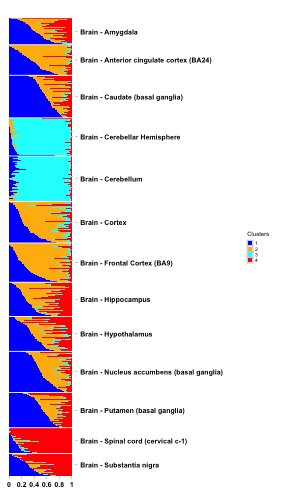
\includegraphics[width=4in,height=6in]{figures/gtex_annot-1}
\end{center}
\end{figure}

\clearpage

\section{Cluster Annotations}

We extract the top genes driving each cluster using the \begin{verb} ExtractTopFeatures() \end{verb} functionality of the \CountClust{} package. We first perform the cluster annotations from the GoM model fit with \Robject{k}=$6$ on the single cell RNA-seq data due to Deng \textit{et al}

\begin{knitrout}
\definecolor{shadecolor}{rgb}{0.969, 0.969, 0.969}\color{fgcolor}\begin{kframe}
\begin{alltt}
\hlstd{theta_mat} \hlkwb{<-} \hlstd{MouseDeng2014.FitGoM}\hlopt{$}\hlstd{clust_6}\hlopt{$}\hlstd{theta;}
\hlstd{top_features} \hlkwb{<-} \hlkwd{ExtractTopFeatures}\hlstd{(theta_mat,} \hlkwc{top_features}\hlstd{=}\hlnum{100}\hlstd{,}
                                   \hlkwc{method}\hlstd{=}\hlstr{"poisson"}\hlstd{,} \hlkwc{options}\hlstd{=}\hlstr{"min"}\hlstd{);}
\hlstd{gene_list} \hlkwb{<-} \hlkwd{do.call}\hlstd{(rbind,} \hlkwd{lapply}\hlstd{(}\hlnum{1}\hlopt{:}\hlkwd{dim}\hlstd{(top_features}\hlopt{$}\hlstd{indices)[}\hlnum{1}\hlstd{],}
                        \hlkwa{function}\hlstd{(}\hlkwc{x}\hlstd{) deng.gene_names[top_features}\hlopt{$}\hlstd{indices[x,]]))}
\end{alltt}
\end{kframe}
\end{knitrout}

We tabulate the top $5$ genes for these $6$ clusters.

\begin{knitrout}
\definecolor{shadecolor}{rgb}{0.969, 0.969, 0.969}\color{fgcolor}\begin{kframe}
\begin{alltt}
\hlstd{xtable}\hlopt{::}\hlkwd{xtable}\hlstd{(gene_list[,}\hlnum{1}\hlopt{:}\hlnum{5}\hlstd{])}
\end{alltt}
\begin{verbatim}
## % latex table generated in R 3.3.3 by xtable 1.8-2 package
## % Fri Oct 13 12:14:25 2017
## \begin{table}[ht]
## \centering
## \begin{tabular}{rlllll}
##   \hline
##  & 1 & 2 & 3 & 4 & 5 \\ 
##   \hline
## 1 & Timd2 & Isyna1 & Alppl2 & Pramel5 & Hsp90ab1 \\ 
##   2 & Upp1 & Tdgf1 & Aqp8 & Fabp5 & Tat \\ 
##   3 & Actb & Krt18 & Fabp3 & Id2 & Tspan8 \\ 
##   4 & Rtn2 & Ebna1bp2 & Zfp259 & Nasp & Cenpe \\ 
##   5 & LOC100502936 & Bcl2l10 & Tcl1 & E330034G19Rik & Oas1d \\ 
##   6 & Obox3 & Zfp352 & Gm8300 & Usp17l5 & BB287469 \\ 
##    \hline
## \end{tabular}
## \end{table}
\end{verbatim}
\end{kframe}
\end{knitrout}

\begin{table}[ht]
\centering
\begin{tabular}{rlllll}
  \hline
 & 1 & 2 & 3 & 4 & 5 \\
  \hline
1 & Timd2 & Isyna1 & Alppl2 & Pramel5 & Hsp90ab1 \\
  2 & Upp1 & Tdgf1 & Aqp8 & Fabp5 & Tat \\
  3 & Actb & Krt18 & Fabp3 & Id2 & Tspan8 \\
  4 & Rtn2 & Ebna1bp2 & Zfp259 & Nasp & Cenpe \\
  5 & LOC100502936 & Bcl2l10 & Tcl1 & E330034G19Rik & Oas1d \\
  6 & Obox3 & Zfp352 & Gm8300 & Usp17l5 & BB287469 \\
   \hline
\end{tabular}
\end{table}

We next perform the same for the topic model fit on the GTEx V6 Brain samples data with \Robject{k}=$4$ clusters.

\begin{knitrout}
\definecolor{shadecolor}{rgb}{0.969, 0.969, 0.969}\color{fgcolor}\begin{kframe}
\begin{alltt}
\hlstd{theta_mat} \hlkwb{<-} \hlstd{GTExV6Brain.FitGoM}\hlopt{$}\hlstd{theta;}
\hlstd{top_features} \hlkwb{<-} \hlkwd{ExtractTopFeatures}\hlstd{(theta_mat,} \hlkwc{top_features}\hlstd{=}\hlnum{100}\hlstd{,}
                                   \hlkwc{method}\hlstd{=}\hlstr{"poisson"}\hlstd{,} \hlkwc{options}\hlstd{=}\hlstr{"min"}\hlstd{);}
\hlstd{gene_list} \hlkwb{<-} \hlkwd{do.call}\hlstd{(rbind,} \hlkwd{lapply}\hlstd{(}\hlnum{1}\hlopt{:}\hlkwd{dim}\hlstd{(top_features}\hlopt{$}\hlstd{indices)[}\hlnum{1}\hlstd{],}
                        \hlkwa{function}\hlstd{(}\hlkwc{x}\hlstd{) gtex.gene_names[top_features}\hlopt{$}\hlstd{indices[x,]]))}
\end{alltt}
\end{kframe}
\end{knitrout}

The top $3$ genes (ensemble IDs) driving these $4$ clusters.

\begin{knitrout}
\definecolor{shadecolor}{rgb}{0.969, 0.969, 0.969}\color{fgcolor}\begin{kframe}
\begin{alltt}
\hlstd{xtable}\hlopt{::}\hlkwd{xtable}\hlstd{(gene_list[,}\hlnum{1}\hlopt{:}\hlnum{3}\hlstd{])}
\end{alltt}
\end{kframe}
\end{knitrout}

\begin{table}[ht]
\centering
\begin{tabular}{rlll}
  \hline
 & 1 & 2 & 3 \\
  \hline
  1 & ENSG00000120885.15 & ENSG00000130203.5 & ENSG00000131771.9 \\
  2 & ENSG00000171617.9 & ENSG00000160014.12 & ENSG00000154146.8 \\
  3 & ENSG00000112139.10 & ENSG00000139899.6 & ENSG00000008710.13 \\
  4 & ENSG00000197971.10 & ENSG00000266844.1 & ENSG00000237973.1 \\
   \hline
\end{tabular}
\end{table}


\begin{thebibliography}{1}

\bibitem{Pritchard2000}
Pritchard, Jonathan K., Matthew Stephens, and Peter Donnelly.
\newblock Inference of population structure using multilocus genotype data.
\newblock {\textit{Genetics}}. 155.2,  945-959, 200.

\bibitem{Rosenberg2002}
Rosenberg NA, Pritchard JK,  Weber JL, Cann HM,  Kidd KK,  Zhivotovsky LA,  Feldman MW.
\newblock The genetic structure of human populations.
\newblock {\textit{Science}}. 298,  2381-2385, 2002.

\bibitem{Blei2003}
Blei DM,  Ng AY, Jordan MI.
\newblock Latent Dirichlet Allocation.
\newblock {\textit{J. Mach. Learn. Res.}}. 3, 993-1022, 2003.

\bibitem{Taddy2012}
Matt Taddy.
\newblock On Estimation and Selection for Topic Models.
\newblock \textit{AISTATS 2012, JMLR W\&CP 22}.(maptpx R package), 2012.

\bibitem{Jaitin2014}
Jaitin DA,  Kenigsberg E et al.
\newblock Massively Parallel Single-Cell RNA-Seq for Marker-Free Decomposition of Tissues into Cell Types.
\newblock {\textit{Science}}. 343 (6172) 776-779, 2014.

\bibitem{Deng2014}
Deng Q,  Ramskold D,  Reinius B,  Sandberg R.
\newblock Single-Cell RNA-Seq Reveals Dynamic, Random Monoallelic Gene Expression in Mammalian Cells.
\newblock {\textit{Science}}.  343 (6167) 193-196, 2014.

\bibitem{GTEX2013}
The GTEx Consortium.
\newblock The Genotype-Tissue Expression (GTEx) project.
\newblock {\textit{Nature genetics}}. 45(6): 580-585. doi:10.1038/ng.2653, 2013.

\end{thebibliography}

% \bibliography{CountClust/REFERENCES}

\section{Supplementary analysis}

As an additional analysis, we apply the \CountClust{} tools on another single-cell RNA-seq data from mouse spleen due to Jaitin \textit{et al} 2014 \cite{Jaitin2014}. The data had technical effects in the form of \begin{verb} amplification batch \end{verb} which the user may want to correct for.

We first install and load the data.

\begin{knitrout}
\definecolor{shadecolor}{rgb}{0.969, 0.969, 0.969}\color{fgcolor}\begin{kframe}
\begin{alltt}
\hlstd{read.data3} \hlkwb{=} \hlkwa{function}\hlstd{() \{}
  \hlstd{x} \hlkwb{=} \hlkwd{tempfile}\hlstd{()}
  \hlkwd{download.file}\hlstd{(}\hlstr{'https://cdn.rawgit.com/jhsiao999/singleCellRNASeqMouseJaitinSpleen/master/data/MouseJaitinSpleen.rda'}\hlstd{,} \hlkwc{destfile} \hlstd{= x,} \hlkwc{quiet}\hlstd{=}\hlnum{TRUE}\hlstd{)}
  \hlstd{z} \hlkwb{=} \hlkwd{get}\hlstd{(}\hlkwd{load}\hlstd{((x)))}
  \hlkwd{return}\hlstd{(z)}
\hlstd{\}}

\hlstd{MouseJaitinSpleen} \hlkwb{<-} \hlkwd{read.data3}\hlstd{()}

\hlcom{## Alternatively}
\hlcom{# devtools::install_github('jhsiao999/singleCellRNASeqMouseJaitinSpleen')}
\end{alltt}
\end{kframe}
\end{knitrout}

\begin{knitrout}
\definecolor{shadecolor}{rgb}{0.969, 0.969, 0.969}\color{fgcolor}\begin{kframe}
\begin{alltt}
\hlstd{jaitin.counts} \hlkwb{<-} \hlstd{Biobase}\hlopt{::}\hlkwd{exprs}\hlstd{(MouseJaitinSpleen)}
\hlstd{jaitin.meta_data} \hlkwb{<-} \hlstd{Biobase}\hlopt{::}\hlkwd{pData}\hlstd{(MouseJaitinSpleen)}
\hlstd{jaitin.gene_names} \hlkwb{<-} \hlkwd{rownames}\hlstd{(jaitin.counts)}
\end{alltt}
\end{kframe}
\end{knitrout}

Extracting the non-ERCC genes satisfying some quality measures.

\begin{knitrout}
\definecolor{shadecolor}{rgb}{0.969, 0.969, 0.969}\color{fgcolor}\begin{kframe}
\begin{alltt}
\hlstd{ENSG_genes_index} \hlkwb{<-} \hlkwd{grep}\hlstd{(}\hlstr{"ERCC"}\hlstd{, jaitin.gene_names,} \hlkwc{invert} \hlstd{=} \hlnum{TRUE}\hlstd{)}
\hlstd{jaitin.counts_ensg} \hlkwb{<-} \hlstd{jaitin.counts[ENSG_genes_index, ]}
\hlstd{filter_genes} \hlkwb{<-} \hlkwd{c}\hlstd{(}\hlstr{"M34473"}\hlstd{,}\hlstr{"abParts"}\hlstd{,}\hlstr{"M13680"}\hlstd{,}\hlstr{"Tmsb4x"}\hlstd{,}
                  \hlstr{"S100a4"}\hlstd{,}\hlstr{"B2m"}\hlstd{,}\hlstr{"Atpase6"}\hlstd{,}\hlstr{"Rpl23"}\hlstd{,}\hlstr{"Rps18"}\hlstd{,}
                  \hlstr{"Rpl13"}\hlstd{,}\hlstr{"Rps19"}\hlstd{,}\hlstr{"H2-Ab1"}\hlstd{,}\hlstr{"Rplp1"}\hlstd{,}\hlstr{"Rpl4"}\hlstd{,}
                  \hlstr{"Rps26"}\hlstd{,}\hlstr{"EF437368"}\hlstd{)}
\hlstd{fcounts} \hlkwb{<-} \hlstd{jaitin.counts_ensg[} \hlopt{-}\hlkwd{match}\hlstd{(filter_genes,} \hlkwd{rownames}\hlstd{(jaitin.counts_ensg)), ]}
\hlstd{sample_counts} \hlkwb{<-} \hlkwd{colSums}\hlstd{(fcounts)}

\hlstd{filter_sample_index} \hlkwb{<-} \hlkwd{which}\hlstd{(jaitin.meta_data}\hlopt{$}\hlstd{number_of_cells} \hlopt{==} \hlnum{1} \hlopt{&}
                              \hlstd{jaitin.meta_data}\hlopt{$}\hlstd{group_name} \hlopt{==} \hlstr{"CD11c+"} \hlopt{&}
                                 \hlstd{sample_counts} \hlopt{>} \hlnum{600}\hlstd{)}
\hlstd{fcounts.filtered} \hlkwb{<-} \hlstd{fcounts[,filter_sample_index];}
\end{alltt}
\end{kframe}
\end{knitrout}

We filter the metadata likewise

\begin{knitrout}
\definecolor{shadecolor}{rgb}{0.969, 0.969, 0.969}\color{fgcolor}\begin{kframe}
\begin{alltt}
\hlstd{jaitin.meta_data_filtered} \hlkwb{<-} \hlstd{jaitin.meta_data[filter_sample_index, ]}
\end{alltt}
\end{kframe}
\end{knitrout}

We fit the GoM model for \Robject{k}=7 and plot the Structure plot visualization to show that the amplification batch indeed drives the clustering patterns.

\begin{knitrout}
\definecolor{shadecolor}{rgb}{0.969, 0.969, 0.969}\color{fgcolor}\begin{kframe}
\begin{alltt}
\hlkwd{StructureObj}\hlstd{(}\hlkwd{t}\hlstd{(fcounts),}
            \hlkwc{nclus_vec}\hlstd{=}\hlnum{7}\hlstd{,} \hlkwc{tol}\hlstd{=}\hlnum{0.1}\hlstd{,}
             \hlkwc{path_rda}\hlstd{=}\hlstr{"../data/MouseJaitinSpleen.FitGoM.rda"}\hlstd{)}
\end{alltt}
\end{kframe}
\end{knitrout}

\begin{knitrout}
\definecolor{shadecolor}{rgb}{0.969, 0.969, 0.969}\color{fgcolor}\begin{kframe}
\begin{alltt}
\hlkwd{data}\hlstd{(}\hlstr{"MouseJaitinSpleen.FitGoM"}\hlstd{)}
\hlkwd{names}\hlstd{(MouseJaitinSpleen.FitGoM}\hlopt{$}\hlstd{clust_7)}
\end{alltt}
\begin{verbatim}
## [1] "K"     "theta" "omega" "BF"    "D"     "X"
\end{verbatim}
\begin{alltt}
\hlstd{omega} \hlkwb{<-} \hlstd{MouseJaitinSpleen.FitGoM}\hlopt{$}\hlstd{clust_7}\hlopt{$}\hlstd{omega}

\hlstd{amp_batch} \hlkwb{<-} \hlkwd{as.numeric}\hlstd{(jaitin.meta_data_filtered[ ,} \hlstr{"amplification_batch"}\hlstd{])}
\hlstd{annotation} \hlkwb{<-} \hlkwd{data.frame}\hlstd{(}
    \hlkwc{sample_id} \hlstd{=} \hlkwd{paste0}\hlstd{(}\hlstr{"X"}\hlstd{,} \hlkwd{c}\hlstd{(}\hlnum{1}\hlopt{:}\hlkwd{NROW}\hlstd{(omega)) ),}
    \hlkwc{tissue_label} \hlstd{=} \hlkwd{factor}\hlstd{(amp_batch,}
                          \hlkwc{levels} \hlstd{=} \hlkwd{rev}\hlstd{(}\hlkwd{sort}\hlstd{(}\hlkwd{unique}\hlstd{(amp_batch))) ) )}
\end{alltt}
\end{kframe}
\end{knitrout}

\begin{figure}[htp]
\begin{center}
\begin{knitrout}
\definecolor{shadecolor}{rgb}{0.969, 0.969, 0.969}\color{fgcolor}\begin{kframe}
\begin{alltt}
\hlkwd{StructureGGplot}\hlstd{(}\hlkwc{omega} \hlstd{= omega,}
                \hlkwc{annotation} \hlstd{= annotation,}
                \hlkwc{palette} \hlstd{= RColorBrewer}\hlopt{::}\hlkwd{brewer.pal}\hlstd{(}\hlnum{9}\hlstd{,} \hlstr{"Set1"}\hlstd{),}
                \hlkwc{yaxis_label} \hlstd{=} \hlstr{"Amplification batch"}\hlstd{,}
                \hlkwc{order_sample} \hlstd{=} \hlnum{FALSE}\hlstd{,}
                \hlkwc{axis_tick} \hlstd{=} \hlkwd{list}\hlstd{(}\hlkwc{axis_ticks_length} \hlstd{=} \hlnum{.1}\hlstd{,}
                                 \hlkwc{axis_ticks_lwd_y} \hlstd{=} \hlnum{.1}\hlstd{,}
                                 \hlkwc{axis_ticks_lwd_x} \hlstd{=} \hlnum{.1}\hlstd{,}
                                 \hlkwc{axis_label_size} \hlstd{=} \hlnum{7}\hlstd{,}
                                 \hlkwc{axis_label_face} \hlstd{=} \hlstr{"bold"}\hlstd{))}
\end{alltt}
\end{kframe}
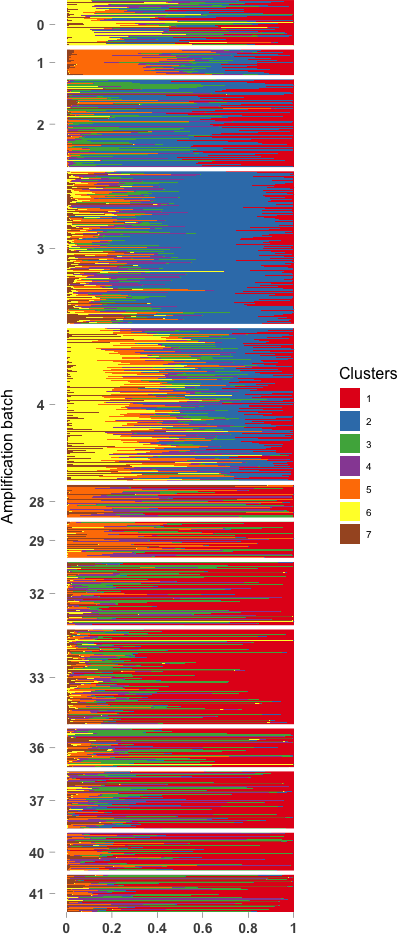
\includegraphics[width=3in,height=7in]{figure/plot_topic-1} 

\end{knitrout}
\end{center}
\end{figure}

It seems from the above Structure plot that \begin{verb} amplification batch \end{verb} drives the clusters. To remove the effect of amplification batch, one can use. For this, we use the \begin{verb} BatchCorrectedCounts() \end{verb} functionality of the package.

\clearpage

\begin{knitrout}
\definecolor{shadecolor}{rgb}{0.969, 0.969, 0.969}\color{fgcolor}\begin{kframe}
\begin{alltt}
\hlstd{batchcorrect.fcounts} \hlkwb{<-} \hlkwd{BatchCorrectedCounts}\hlstd{(}\hlkwd{t}\hlstd{(fcounts.filtered),}
                                          \hlstd{amp_batch,} \hlkwc{use_parallel} \hlstd{=} \hlnum{FALSE}\hlstd{);}
\hlkwd{dim}\hlstd{(batchcorrect.fcounts)}
\end{alltt}
\end{kframe}
\end{knitrout}

\section{Acknowledgements}

We would like to thank Deng \textit{et al} and the GTEx Consortium for having making the data publicly available. We would like to thank Matt Taddy, Amos Tanay, Po Yuan Tung and Raman Shah for helpful discussions related to the project and the package.

\section{Session Info}

\begin{knitrout}
\definecolor{shadecolor}{rgb}{0.969, 0.969, 0.969}\color{fgcolor}\begin{kframe}
\begin{alltt}
\hlkwd{sessionInfo}\hlstd{()}
\end{alltt}
\begin{verbatim}
## R version 3.3.3 (2017-03-06)
## Platform: x86_64-apple-darwin13.4.0 (64-bit)
## Running under: macOS Sierra 10.12.5
## 
## locale:
## [1] en_US.UTF-8/en_US.UTF-8/en_US.UTF-8/C/en_US.UTF-8/en_US.UTF-8
## 
## attached base packages:
## [1] stats     graphics  grDevices utils     datasets  methods   base     
## 
## other attached packages:
## [1] CountClust_0.1.2 ggplot2_2.2.1    devtools_1.13.3  knitr_1.16      
## 
## loaded via a namespace (and not attached):
##  [1] Rcpp_0.12.12        RColorBrewer_1.1-2  git2r_0.18.0       
##  [4] plyr_1.8.4          highr_0.6           tools_3.3.3        
##  [7] boot_1.3-18         digest_0.6.12       nlme_3.1-131       
## [10] evaluate_0.10       memoise_1.1.0       tibble_1.3.4       
## [13] gtable_0.2.0        lattice_0.20-34     mgcv_1.8-17        
## [16] rlang_0.1.1.9000    Matrix_1.2-10       curl_2.6           
## [19] parallel_3.3.3      cluster_2.0.5       withr_1.0.2        
## [22] httr_1.2.1          stringr_1.2.0       gtools_3.5.0       
## [25] stats4_3.3.3        grid_3.3.3          nnet_7.3-12        
## [28] cowplot_0.8.0       Biobase_2.34.0      R6_2.2.2           
## [31] maptpx_1.9-3        flexmix_2.3-14      limma_3.30.13      
## [34] reshape2_1.4.2.9000 magrittr_1.5        BiocGenerics_0.20.0
## [37] MASS_7.3-45         scales_0.4.1        modeltools_0.2-21  
## [40] xtable_1.8-2        permute_0.9-4       ape_4.1            
## [43] BiocStyle_2.2.1     picante_1.6-2       colorspace_1.3-2   
## [46] stringi_1.1.5       lazyeval_0.2.0      munsell_0.4.3      
## [49] slam_0.1-40         SQUAREM_2017.10-1   vegan_2.4-3
\end{verbatim}
\end{kframe}
\end{knitrout}

\end{document}
